% !Mode:: "TeX:UTF-8"
\documentclass[aspectratio=169,12pt]{beamer}

% 主题设置
\usetheme{Madrid}
\usecolortheme{seahorse}

% 中文支持
\usepackage{xeCJK}
\usepackage{fontspec}
\setCJKmainfont{Noto Sans CJK SC}
\setmainfont{Liberation Serif}

% 数学符号
\usepackage{amsmath,amssymb,amsthm}

% 图形支持
\usepackage{graphicx}
\usepackage{tikz}

% 表格
\usepackage{booktabs}
\usepackage{array}
\usepackage{multirow}

% 算法
\usepackage{algorithm}
\usepackage{algorithmic}

% 其他包
\usepackage{xcolor}
\usepackage{hyperref}

% 自定义颜色(常见Beamer学术蓝灰配色)
\definecolor{hitblue}{RGB}{0,63,114}
\definecolor{hitgray}{RGB}{74,85,104}

% 统一Beamer配色
\setbeamercolor{structure}{fg=hitblue}
\setbeamercolor{palette primary}{fg=white,bg=hitblue}
\setbeamercolor{palette secondary}{fg=white,bg=hitgray}
\setbeamercolor{frametitle}{fg=white,bg=hitblue}
\setbeamercolor{title}{fg=white}

\setbeamercolor{block title}{fg=white,bg=hitblue}
\setbeamercolor{block body}{fg=black,bg=hitblue!6}
\setbeamercolor{alertblock title}{fg=white,bg=hitgray}
\setbeamercolor{alertblock body}{fg=black,bg=hitgray!10}
\setbeamercolor{exampleblock title}{fg=white,bg=hitblue!85!black}
\setbeamercolor{exampleblock body}{fg=black,bg=hitblue!8}
\setbeamercolor{alerted text}{fg=hitgray}

% 标题页信息
\title[面向人脸识别模型的逆向重建方法研究]{面向人脸识别模型的逆向重建方法研究}
\subtitle{硕士学位论文答辩}
\author[俞磊]{俞磊}
\institute[HIT]{哈尔滨工业大学\\网络空间安全学院}
\date{\today}

% 自定义命令
% 字体大小选项(从大到小):
% \Huge > \huge > \LARGE > \Large > \large > \normalsize(默认)> \small > \footnotesize > \scriptsize > \tiny

% 重定义粗体命令为学术蓝色
\renewcommand{\textbf}[1]{\textcolor{hitblue}{\bfseries #1}}

\newcommand{\highlight}[1]{\textcolor{hitblue}{\textbf{#1}}}
\newcommand{\important}[1]{\textcolor{hitgray}{\textbf{#1}}}

\begin{document}

% 标题页
\begin{frame}[plain]
\titlepage
\end{frame} % 标题页

% 目录
\begin{frame}{目录}
\begin{enumerate}
  \item \textbf{研究背景与威胁建模}

  \item \textbf{研究内容与主要方法}

  \item \textbf{基于角度约束对比学习的模板逆向重建方法设计与验证}

  \item \textbf{基于换脸先验迁移的多目标自适应模型反演方法设计与验证}

  \item \textbf{结论与防御措施讨论}

  \item \textbf{评阅意见及相应修改}
\end{enumerate}
\end{frame} % 目录

\section{研究背景与意义}

\begin{frame}{研究背景}
\footnotesize
\begin{columns}[c]
\begin{column}{0.48\textwidth}
\textbf{人脸识别系统的广泛部署}
\begin{itemize}\setlength{\itemsep}{1pt}
  \item 深度神经网络驱动的人脸识别已深度渗透至\important{身份认证、公共安全、金融支付、门禁控制}等安全敏感场景
  \item 广泛部署在带来便捷性的同时,也使海量用户的生物特征模板成为攻击者的重要目标
\end{itemize}

\vspace{2pt}
\textbf{两类系统架构 $\Rightarrow$ 两类攻击面}

\begin{itemize}\setlength{\itemsep}{1pt}
  \item \important{检索型架构:}特征模板长期存于数据库,泄露后可被\textbf{TIA}利用,从嵌入向量重建人脸图像
  \item \important{分类型架构:}输出置信度/概率分布包含丰富语义,可被\textbf{MIA}利用,从类别标签重建训练样本
\end{itemize}
\end{column}

\begin{column}{0.50\textwidth}
\textbf{逆向重建技术的演进脉络}

\begin{itemize}\setlength{\itemsep}{1pt}
  \item \important{优化类方法:}迭代梯度下降,计算开销大、易陷局部极值,生成质量差
  \item \important{GAN类方法:}引入生成先验,但训练不稳定且存在模式崩塌问题
  \item \important{扩散模型方法:}训练稳定、模式覆盖全面,高保真重建
\end{itemize}

\end{column}
\end{columns}
\end{frame} % 研究背景

\section{研究内容与方法}

\begin{frame}{研究问题、威胁与方案概述}
\footnotesize
\begin{columns}[T]
\begin{column}{0.5\textwidth}
\textbf{模板逆向攻击(TIA)—— 第3章}
\begin{itemize}\setlength{\itemsep}{1pt}
  \item \important{威胁场景:}检索型系统数据库泄露/内部威胁,攻击者获取模板 $t\!=\!F(x_0)$
  \item \important{攻击目标:}构造 $\hat{x}\!=\!g(t)$ 满足 $\mathrm{sim}(F(\hat{x}),t)>\tau$ 且 $\hat{x}\!\in\!\mathcal{M}_{\text{nat}}$
  \item \important{关键瓶颈:}
    {\scriptsize\begin{itemize}\setlength{\itemsep}{0pt}
      \item 维度压缩 $d\!\ll\!HWC$,逆映射多对一、欠定无唯一解
      \item 超球面几何与连续嵌入引导机制适配不足
    \end{itemize}}
  \item \important{本文方案:}{\scriptsize \textbf{EDM} + \textbf{角度约束对比学习} + \textbf{任务不确定性加权} + \textbf{梯度引导推理}}
\end{itemize}
\end{column}
\begin{column}{0.5\textwidth}
\textbf{模型反演攻击(MIA)—— 第4章}
\begin{itemize}\setlength{\itemsep}{1pt}
  \item \important{威胁场景:}分类型系统白盒访问,攻击者仅持有类别标签 $y$,无任何原始图像
  \item \important{攻击目标:}构造 $\hat{x}$ 满足 $F_\theta(\hat{x})_y>\tau$ 且 $\hat{x}\!\in\!\mathcal{M}_{\text{nat}}$
  \item \important{关键瓶颈:}
    {\scriptsize\begin{itemize}\setlength{\itemsep}{0pt}
      \item 换脸先验依赖真实目标图像,与离散标签输入模态根本不兼容
      \item 标签嵌入分布与ArcFace身份嵌入分布存在显著偏移
    \end{itemize}}
  \item \important{本文方案:}{\scriptsize \textbf{REFace先验} + \textbf{标签条件嵌入层} + \textbf{LoRA微调} + \textbf{三阶段渐进训练}}
\end{itemize}
\end{column}
\end{columns}
\end{frame} % 研究问题威胁与方案概述

\section{基于角度约束对比学习的模板逆向重建方法设计与验证}

\begin{frame}{TIA问题定义与关键挑战}
\footnotesize
\begin{columns}[T]
\begin{column}{0.5\textwidth}
\textbf{攻击威胁模型}\\[2pt]
特征提取器 $F\!:\mathbb{R}^{HWC}\!\to\!\mathbb{R}^d$ 将图像映射至低维嵌入。攻击者通过数据库泄露获取模板 $t=F(x_0)$,目标为逆映射 $\hat{x}=g(t)$:
\vspace{-4pt}
{\scriptsize\begin{equation*}
\hat{x}=\arg\min_x\,\mathcal{L}_{emb}(F(x),t)+\lambda_p\mathcal{L}_{perc}(x)+\lambda_r R(x),\;\text{s.t.}\;\hat{x}\!\in\!\mathcal{M}_{nat}
\end{equation*}}\vspace{-4pt}
\textbf{攻击成功判据(三层次)}
\begin{itemize}\setlength{\itemsep}{1pt}
  \item \important{强成功:}$\mathrm{sim}(F(\hat{x}),t)\geq\tau$,直接通过身份验证
  \item \important{弱成功:}相似度显著高于随机基线,部分泄露身份信息
  \item \important{视觉成功:}生成自然人脸外观,通过人类视觉检验
\end{itemize}
\end{column}
\begin{column}{0.5\textwidth}
\textbf{核心挑战}
\begin{itemize}\setlength{\itemsep}{2pt}
  \item \important{逆问题求解:}$d\!\ll\!HWC$ 导致逆映射多对一,无唯一解
  \item \important{特征空间不同:}ArcFace余弦度量空间与传统欧氏优化方向不一致
  \item \important{协同优化:}生成先验视觉真实性目标与特征空间身份约束存在优化冲突
  \item \important{权重平衡:}多目标损失(像素/特征)相对权重缺乏自动化调节机制
\end{itemize}
\end{column}
\end{columns}
\end{frame} % 模板逆向·问题定义与关键挑战

\begin{frame}{基于角度约束对比学习的模板逆向重建方法整体架构}
\begin{columns}[c]
\begin{column}{0.5\textwidth}
\scalebox{0.45}{%
\begin{tikzpicture}[node distance=1.5cm, >=stealth, thick,
  module/.style={rectangle, draw=blue!60, fill=blue!10, minimum width=3.2cm, minimum height=0.9cm, align=center, rounded corners},
  input/.style={rectangle, draw=green!60, fill=green!10, minimum width=2.2cm, minimum height=0.7cm, align=center, rounded corners},
  loss/.style={rectangle, draw=red!60, fill=red!10, minimum width=2.3cm, minimum height=0.7cm, align=center, rounded corners},
  arrow/.style={->, thick},
  gradient/.style={->, thick, dashed, red!70}]
  \node[input] (x) at (0,0) {原始图像 $x$};
  \node[input] (t) at (6,0) {目标模板 $t$};
  \node[module] (diffusion) at (0,-2.2) {扩散去噪网络 \\ $f_\theta$ (EDM)};
  \node[module] (recognizer) at (6,-2.2) {特征提取器 \\ $F$ (ArcFace)};
  \node[input] (x0) at (0,-4) {生成图像 $\hat{x}_0$};
  \node[input] (feat) at (6,-4) {特征 $F(\hat{x}_0)$};
  \node[loss] (pixel) at (0,-5.8) {$\mathcal{L}_{\text{pixel}}$};
  \node[loss] (angular) at (3,-5.8) {$\mathcal{L}_{\text{feat}}$};
  \node[loss] (div) at (6,-5.8) {$\mathcal{L}_{\text{div}}$};
  \node[loss] (total) at (3,-7.3) {$\mathcal{L}_{\text{total}}$ (加权)};
  \draw[arrow] (x) -- (diffusion);
  \draw[arrow] (diffusion) -- (x0);
  \draw[arrow] (t) -- (recognizer);
  \draw[arrow] (recognizer) -- (feat);
  \draw[arrow] (x) -- ++(1.8,0) |- (recognizer);
  \draw[arrow] (x0) -- ++(2.2,0) |- (recognizer);
  \draw[arrow] (x0) -- (pixel);
  \draw[arrow] (feat) -- (angular);
  \draw[arrow] (feat) -- (div);
  \draw[arrow] (pixel) -- (total);
  \draw[arrow] (angular) -- (total);
  \draw[arrow] (div) -- (total);
  \draw[gradient, rounded corners=5pt] (total.south) -- ++(0,-0.5) -| ([xshift=-3cm]diffusion.west) -- (diffusion.west);
\end{tikzpicture}}
\end{column}
\begin{column}{0.5\textwidth}
\footnotesize\textbf{核心设计}
\begin{itemize}\setlength{\itemsep}{0pt}
  \item \highlight{EDM生成骨干:}去噪先验天然保证生成样本位于 $\mathcal{M}_{nat}$,从根本上解决视觉真实性
  \item \highlight{角度约束对比学习 $\mathcal{L}_{feat}$:}利用ArcFace超球面几何拉近正样本、拉远负样本,与识别器决策边界精确对齐
  \item \highlight{多样性约束 $\mathcal{L}_{div}$:}最大化批内样本角度距离,防止模式崩塌
  \item \highlight{任务不确定性加权:}$\sigma_p,\sigma_f$ 与 $\theta$ 联合优化,自动平衡像素与特征权重
\end{itemize}
{\scriptsize\begin{equation*}
\mathcal{L}=\frac{\mathcal{L}_{pixel}}{2\sigma_p^2}+\frac{\mathcal{L}_{feat}}{2\sigma_f^2}+\frac{1}{2}(\log\sigma_p^2+\log\sigma_f^2)-\beta\mathcal{L}_{div}
\end{equation*}}
\end{column}
\end{columns}
\end{frame} % 方法整体架构与核心设计

\begin{frame}{训练策略与推理流程}
\begin{columns}[T]
\begin{column}{0.50\textwidth}
\centering\footnotesize\textbf{训练流程}\\[2pt]
\includegraphics[width=\linewidth,height=0.32\textheight,keepaspectratio]{figures/train-1.pdf}\\[4pt]
\textbf{推理流程}\\[2pt]
\includegraphics[width=\linewidth,height=0.32\textheight,keepaspectratio]{figures/infer.pdf}
\end{column}
\begin{column}{0.50\textwidth}
\footnotesize\textbf{两阶段训练策略}
\begin{itemize}\setlength{\itemsep}{2pt}
  \item \important{预热阶段}:仅优化 $\mathcal{L}_{pixel}$,建立稳定人脸流形去噪先验
  \item \important{主训练阶段}:启用完整 $\mathcal{L}$,初始 $\log\sigma_p\!=\!\log\sigma_f\!=\!0$,$\theta,\sigma_p,\sigma_f$ 联合更新;训练后期 $\sigma_f<\sigma_p$,特征匹配权重自动增大
\end{itemize}
\vspace{4pt}
\textbf{模板条件梯度引导推理}\\[2pt]
{\scriptsize\begin{equation*}
x_{i-1}=x_i+(\sigma_{i-1}\!-\!\sigma_i)\!\left[\underbrace{\frac{f_\theta(x_i,t,\sigma_i)-x_i}{\sigma_i}}_{\text{去噪方向}}+\underbrace{\alpha\nabla_{x_i}\mathrm{sim}(F(x_i),t)}_{\text{模板引导}}\right]
\end{equation*}}
{\scriptsize 引导强度 $\alpha$ 权衡生成质量与特征匹配度,训练与推理形成一致闭环}
\end{column}
\end{columns}
\end{frame} % 训练策略与推理流程


\begin{frame}{实验结果}
\begin{columns}[T]
\begin{column}{0.5\textwidth}
\footnotesize\textbf{实验设置}
\begin{itemize}\setlength{\itemsep}{1pt}
  \item 训练:CelebA(202,599)
  \item 测试:MOBIO / LFW / AgeDB / IJB-C
  \item 目标:ArcFace(512维,白盒)
  \item 指标:SAR@FMR=$10^{-2}/10^{-3}$、FID、ID-Pres
\end{itemize}
\vspace{4pt}
\footnotesize\textbf{LFW基准对比}\\[2pt]
{\scriptsize\begin{tabular}{lcccc}
\toprule
\textbf{方法} & \textbf{SAR@$10^{-2}$} & \textbf{SAR@$10^{-3}$} & \textbf{FID↓} & \textbf{ID↑} \\
\midrule
GaFaR        & 89.41 & 79.97 & 32.1 & 0.834 \\
Shahreza     & 92.47 & \textbf{85.14} & 28.5 & 0.891 \\
\textbf{本文} & \textbf{94.23} & 84.23 & \textbf{18.27} & \textbf{0.947} \\
\bottomrule
\end{tabular}}
\end{column}
\begin{column}{0.5\textwidth}
\footnotesize\textbf{跨数据集结果(SAR, \%)}\\[2pt]
{\scriptsize\begin{tabular}{lcccc}
\toprule
 & \textbf{MOBIO} & \textbf{LFW} & \textbf{AgeDB} & \textbf{IJB-C} \\
\midrule
\multicolumn{5}{c}{\textit{FMR=$10^{-2}$}} \\
GaFaR        & 95.84 & 89.41 & 63.45 & 69.32 \\
Shahreza     & 96.53 & 92.47 & 73.91 & 78.62 \\
\textbf{本文} & \textbf{97.38} & \textbf{94.23} & \textbf{75.64} & \textbf{82.91} \\
\multicolumn{5}{c}{\textit{FMR=$10^{-3}$}} \\
GaFaR        & 82.93 & 79.97 & 49.08 & 29.91 \\
Shahreza     & 84.89 & \textbf{85.14} & 60.18 & 45.57 \\
\textbf{本文} & \textbf{87.87} & 84.23 & \textbf{65.81} & \textbf{55.58} \\
\bottomrule
\end{tabular}}
\end{column}
\end{columns}
\end{frame} % 模板逆向·实验结果

\begin{frame}{实验结果}
\begin{columns}[T]
\begin{column}{0.44\textwidth}
\centering
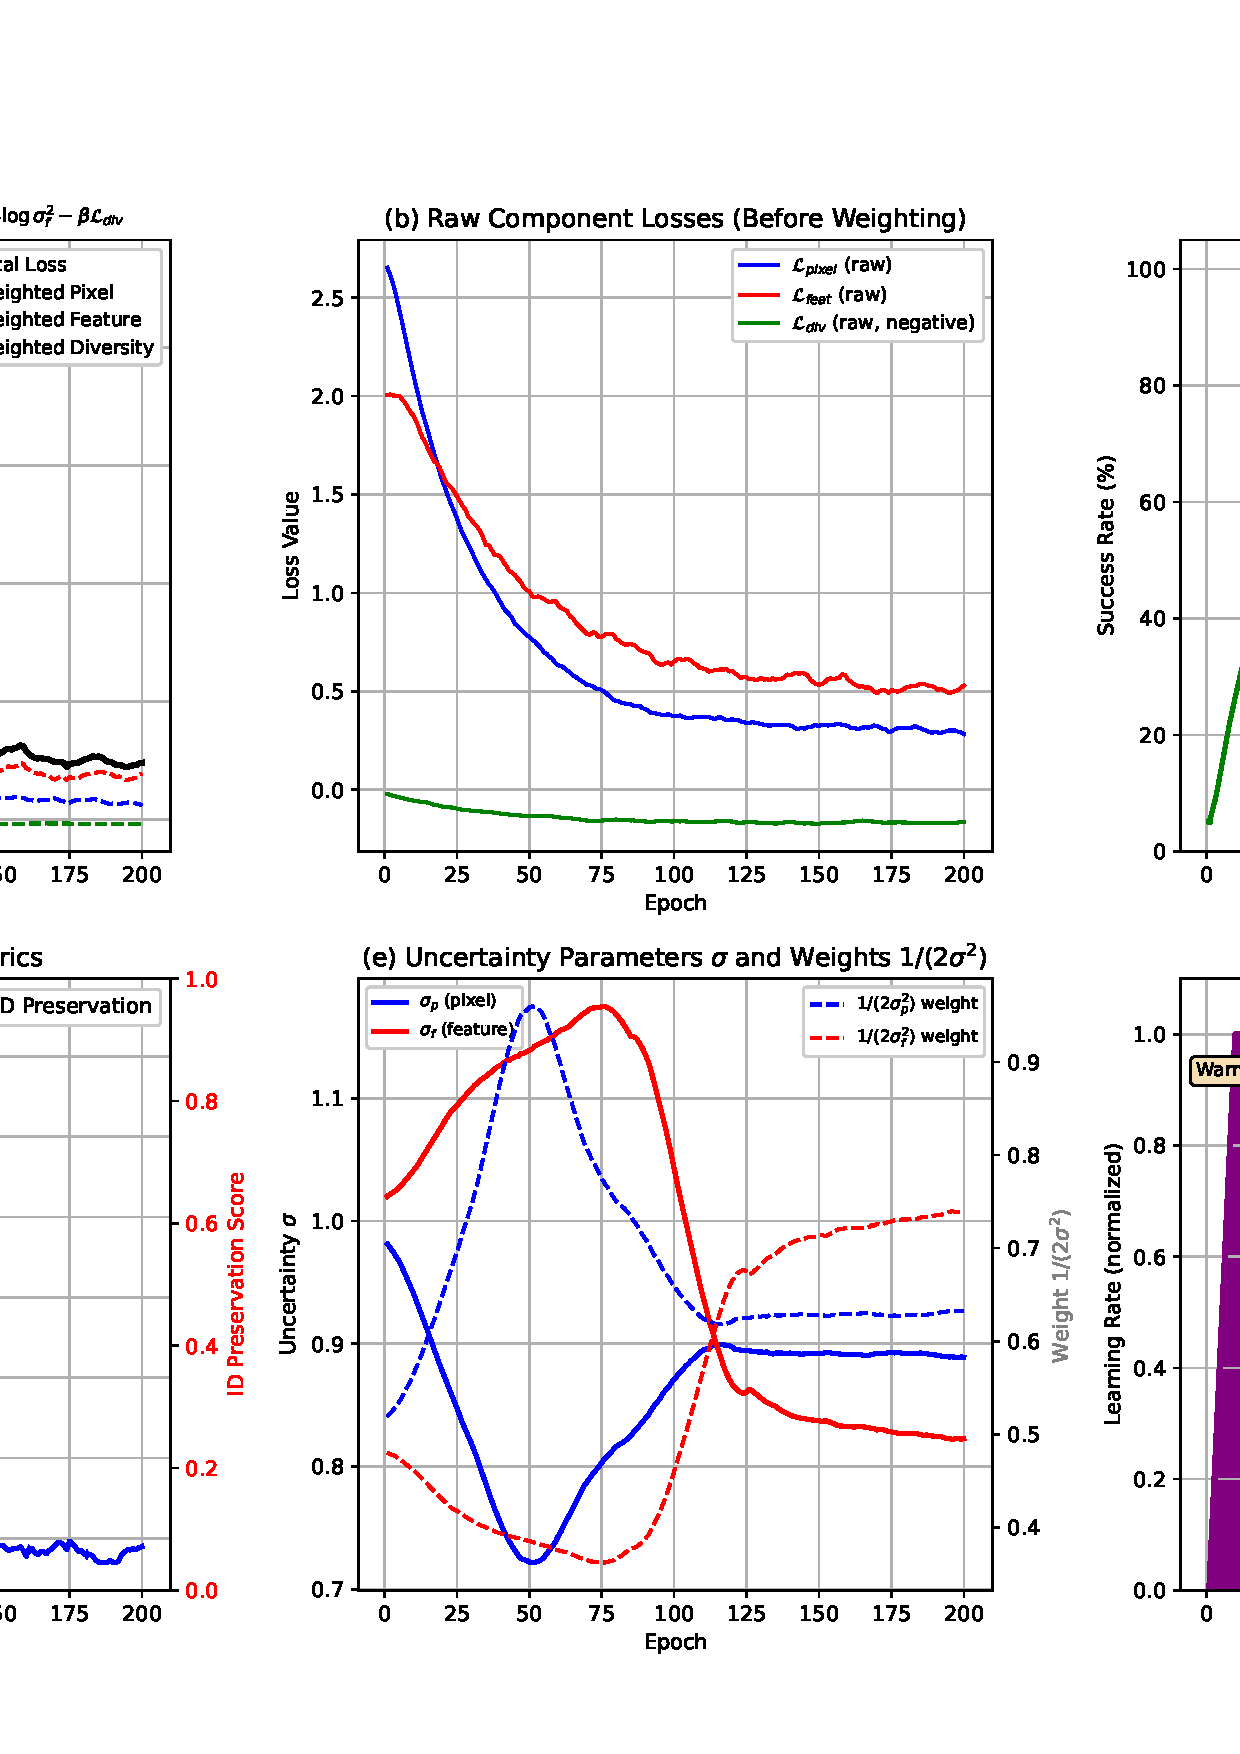
\includegraphics[width=\linewidth,height=0.5\textheight,keepaspectratio]{figures/tia_training_curves.pdf}\\
\vspace{4pt}
\includegraphics[width=\linewidth,height=0.4\textheight,keepaspectratio]{figures/matrix_3x10.png}\\
{\scriptsize 真实/重建/Grad-CAM}
\end{column}
\begin{column}{0.54\textwidth}
\footnotesize 消融结果:\\[8pt]
{\resizebox{\linewidth}{!}{\begin{tabular}{lcccc}
\hline
\textbf{模型配置} & \textbf{SAR@$10^{-2}$} & \textbf{SAR@$10^{-3}$} & \textbf{FID↓} & \textbf{ID↑} \\
\hline
$\mathcal{L}_{\text{pixel}}$ & 68.33\% & 41.67\% & 52.46 & 0.703 \\
$\mathcal{L}_{\text{pixel}} + \mathcal{L}_{\text{feat}}$ & 91.33\% & 79.83\% & 32.18 & 0.891 \\
$\mathcal{L}_{\text{pixel}} + \mathcal{L}_{\text{feat}} + $ 不确定性加权 & 92.83\% & 82.17\% & 27.54 & 0.923 \\
\textbf{$\mathcal{L}_{\text{pixel}} + \mathcal{L}_{\text{feat}} + $ 不确定性加权 $ + \mathcal{L}_{\text{div}}$} & \textbf{94.23\%} & \textbf{84.23\%} & \textbf{18.27} & \textbf{0.947} \\
\hline
\end{tabular}}}
\vspace{12pt}
\begin{block}{}\scriptsize
\textbf{可视化:}重建与目标高度一致;热力图激活集中于眼鼻嘴,验证超球面对齐有效性。\\[2pt]
\textbf{消融:}$\mathcal{L}_{\text{feat}}$贡献最大(+38.16ppt);$\mathcal{L}_{\text{div}}$对FID降幅最显著($-$9.27);训练曲线三阶段收敛稳定。
\end{block}
\end{column}
\end{columns}
\end{frame} % 模板逆向·可视化与消融实验

\section{基于换脸先验迁移的多目标自适应模型反演方法设计与验证}

\begin{frame}{模型反演·问题定义与核心挑战}
\small
\textbf{目标:}仅给定类别标签$y$,生成样本$\hat{x}$,使其同时满足:
\begin{itemize}
  \item \textbf{攻击有效性:}被目标分类器高置信识别为$y$
  \item \textbf{视觉真实性:}保持自然人脸纹理与结构
\end{itemize}

\begin{block}{核心矛盾(第4章)}
\begin{enumerate}
  \item 换脸模型原生依赖\textbf{目标图像条件},攻击场景只有\textbf{离散标签}
  \item 标签嵌入分布与ArcFace真实身份嵌入分布存在偏移
  \item 分类器攻击目标与生成保真目标需要动态平衡
\end{enumerate}
\end{block}

\begin{alertblock}{一句话结论}
MIA的关键是将“标签条件”稳定迁移到“换脸先验”的身份控制通道。
\end{alertblock}
\end{frame} % 模型反演·问题定义与核心挑战

\begin{frame}{模型反演·核心设计要点}
\small
\begin{itemize}
  \item \highlight{换脸先验(REFace):}利用身份-属性显式解耦机制,将身份嵌入通过交叉注意力注入去噪过程;相比类条件生成,具备更丰富的面部结构与纹理先验,且无需从零训练
  \item \highlight{标签条件嵌入层:}多层感知机将独热编码$y$映射为归一化身份嵌入$e_{id}\in\mathbb{R}^{512}$,无缝替代REFace原有的ArcFace图像编码器,建立离散标签到连续嵌入的可学习桥梁
  \item \highlight{LoRA参数高效微调($r{=}16,\alpha{=}32$):}仅训练主干1\%--5\%参数,在冻结预训练权重的同时适配新嵌入分布,有效避免过拟合
  \item \highlight{六类损失函数:}扩散先验$\mathcal{L}_{prior}$、分类引导$\mathcal{L}_{cls}$(top-k margin)、特征正则$\mathcal{L}_{p\text{-}reg}$、身份一致性$\mathcal{L}_{id}$、感知质量$\mathcal{L}_{perc}$(LPIPS)、参数正则$\mathcal{L}_{reg}$;任务不确定性加权自动整合
  \item \highlight{三阶段渐进训练:}(1)图像条件预热$\to$(2)余弦退火混合条件过渡$\to$(3)纯标签条件适配,实现从换脸先验到MIA攻击的平滑模态迁移
\end{itemize}
\end{frame} % 模型反演·核心设计要点

\begin{frame}{模型反演·方法架构}
\begin{columns}[T]
  \column{0.52\textwidth}
  \centering\small\textbf{方法整体架构}\\[2pt]
  \scalebox{0.36}{%
  \begin{tikzpicture}[scale=0.75, transform shape, node distance=1.3cm, >=stealth, thick,
    module/.style={rectangle, draw=blue!60, fill=blue!10, minimum width=2.5cm, minimum height=0.75cm, align=center, rounded corners},
    input/.style={rectangle, draw=green!60, fill=green!10, minimum width=1.8cm, minimum height=0.6cm, align=center, rounded corners},
    submodule/.style={rectangle, draw=purple!60, fill=purple!10, minimum width=2.2cm, minimum height=0.6cm, align=center, rounded corners, font=\small},
    loss/.style={rectangle, draw=red!60, fill=red!10, minimum width=1.6cm, minimum height=0.55cm, align=center, rounded corners, font=\small},
    arrow/.style={->, thick},
    gradient/.style={->, thick, dashed, red!70}]
    \node[input] (label) at (0,0) {目标类别};
    \node[input] (src) at (8,0) {源图像};
    \node[module] (embed) at (0,-1.6) {嵌入层 $\mathcal{E}_\psi$};
    \node[input] (eid) at (0,-3) {$e_{\text{id}}$};
    \node[submodule] (vae_enc) at (8,-1.6) {VAE编码器};
    \node[submodule] (unet) at (8,-3) {U-Net + LoRA};
    \node[submodule] (vae_dec) at (8,-4.4) {VAE解码器};
    \node[input] (xhat) at (4,-6) {生成图像 $\hat{x}$};
    \node[module] (arcface) at (2,-7.5) {ArcFace $E_{\text{id}}$};
    \node[module] (classifier) at (6.5,-7.5) {分类器 $F_\theta$};
    \node[input] (feat_gen) at (2,-8.8) {$e_{\text{gen}}$};
    \node[input] (logits) at (5.7,-8.8) {logits};
    \node[input] (feat_cls) at (7.3,-8.8) {特征};
    \node[loss] (loss_reg) at (-3,-3.5) {$\mathcal{L}_{\text{reg}}$};
    \node[loss] (loss_prior) at (10.5,-4) {$\mathcal{L}_{\text{prior}}$};
    \node[loss] (loss_perc) at (4,-9.8) {$\mathcal{L}_{\text{perc}}$};
    \node[loss] (loss_id) at (2,-10) {$\mathcal{L}_{\text{id}}$};
    \node[loss] (loss_cls) at (5.7,-10) {$\mathcal{L}_{\text{cls}}$};
    \node[loss] (loss_preg) at (7.3,-10) {$\mathcal{L}_{\text{p-reg}}$};
    \node[loss, minimum width=2cm] (total) at (4,-11.8) {$\mathcal{L}_{\text{total}}$ (任务不确定性加权)};
    \draw[arrow] (label) -- (embed);
    \draw[arrow] (embed) -- (eid);
    \draw[arrow] (src) -- (vae_enc);
    \draw[arrow] (vae_enc) -- (unet);
    \draw[arrow] (unet) -- (vae_dec);
    \draw[arrow] (vae_dec) -- (xhat);
    \draw[arrow] (xhat) -| (arcface);
    \draw[arrow] (xhat) -| (classifier);
    \draw[arrow] (arcface) -- (feat_gen);
    \draw[arrow] (classifier.south) -- ++(0,-0.4) -| (logits.north);
    \draw[arrow] (classifier.south) -- ++(0,-0.4) -| (feat_cls.north);
    \draw[arrow] (eid.east) -| ([xshift=-1.2cm]unet.west) -- (unet.west);
    \draw[arrow] (embed.west) -| (loss_reg);
    \draw[arrow] (unet.east) -| (loss_prior);
    \draw[arrow] (xhat) -- (loss_perc);
    \draw[arrow] (feat_gen) -- (loss_id);
    \draw[arrow] (eid) -- ++(-1.5,0) |- (loss_id);
    \draw[arrow] (logits) -- (loss_cls);
    \draw[arrow] (feat_cls) -- (loss_preg);
    \draw[arrow] (loss_reg) |- (total);
    \draw[arrow] (loss_prior) |- (total);
    \draw[arrow] (loss_perc) -- (total);
    \draw[arrow] (loss_id) -- (total);
    \draw[arrow] (loss_cls) -- (total);
    \draw[arrow] (loss_preg) |- (total);
    \draw[gradient, rounded corners=8pt] (total) -- ++(0,-0.8) -| ([xshift=3cm]unet.east) -- (unet.east);
    \draw[gradient, rounded corners=8pt] (total) -- ++(0,-0.8) -| ([xshift=-3.5cm]embed.west) -- (embed.west);
  \end{tikzpicture}}

  \column{0.46\textwidth}
  \centering\small\textbf{三阶段训练流程}\\[2pt]
  \includegraphics[width=\linewidth]{figures/train_mia.pdf}
\end{columns}
\end{frame} % 模型反演·方法架构

\begin{frame}{模型反演·多目标损失设计}
\small
\begin{columns}[T]
  \column{0.52\textwidth}
  \textbf{六类损失(第4章)}
  \begin{itemize}
    \item 扩散先验:$\mathcal{L}_{prior}$
    \item 分类引导(top-k margin):$\mathcal{L}_{cls}$
    \item 特征正则(p-reg):$\mathcal{L}_{p-reg}$
    \item 身份一致性对比:$\mathcal{L}_{id}$
    \item 感知质量(LPIPS):$\mathcal{L}_{perc}$
    \item 嵌入/LoRA正则:$\mathcal{L}_{reg}$
  \end{itemize}

  \column{0.46\textwidth}
  \begin{block}{任务不确定性加权}
  \small
  \[
  \mathcal{L}_{total}=\sum_i\left(\frac{1}{2\sigma_i^2}\mathcal{L}_i+\frac{1}{2}\log\sigma_i^2\right)
  \]
  \normalsize
  自动学习各任务权重,减少人工调参依赖。
  \end{block}
\end{columns}

\begin{alertblock}{一句话结论}
通过自适应加权,MIA在“攻击强度”和“生成质量”之间实现动态平衡。
\end{alertblock}
\end{frame} % 模型反演·多目标损失设计

\begin{frame}{模型反演·训练与推理策略}
\small
\begin{columns}[T]
  \column{0.47\textwidth}
  \textbf{三阶段渐进训练}\\[3pt]
  \textbf{阶段1:图像条件预热}\\{\footnotesize 仅训 LoRA,稳定换脸生成能力}
  \\[3pt]
  \textbf{阶段2:混合条件过渡}\\{\footnotesize $e_{id}=(1-\lambda)E_{id}(x_{real})+\lambda\mathcal{E}_\psi(y)$,余弦退火平滑迁移}
  \\[3pt]
  \textbf{阶段3:纯标签条件适配}\\{\footnotesize 始用分类器引导,优化攻击有效性+身份一致性}
  \\[4pt]
  \begin{block}{论文对应结果}
  {\footnotesize 三阶段将TarAcc:70.85\%\ $\to$\ 94.87\%,FID:43.21\ $\to$\ 23.26}
  \end{block}

  \column{0.5\textwidth}
  \centering\small\textbf{分类器引导推理流程}\\[2pt]
  \includegraphics[width=\linewidth]{figures/infer_mia-1.pdf}
\end{columns}
\end{frame} % 模型反演·训练与推理策略

\begin{frame}{模型反演·实验结果}
\footnotesize
\begin{columns}[T]
  \column{0.44\textwidth}
  \textbf{实验设置}
  \begin{itemize}\setlength{\itemsep}{1pt}
    \item 目标任务:VGGFace2(1000类)
    \item 目标分类器:ArcFace / IR152 / Face.evoLVe
    \item 辅助数据:CelebA、FaceScrub
    \item LoRA:$r{=}16,\alpha{=}32$,AdamW
    \item 指标:TarAcc、EvalAcc、FID、KNN
  \end{itemize}
  \vspace{3pt}
  \textbf{基准对比(VGGFace2, ArcFace)}\\[2pt]
  {\scriptsize\begin{tabular}{lcccc}
  \toprule
  \textbf{方法} & \textbf{TarAcc↑} & \textbf{EvalAcc↑} & \textbf{FID↓} & \textbf{KNN↑} \\
  \midrule
  GMI     & 28.52\% & 1.38\%  & 24.87 & 0.559 \\
  PLG-MI  & 40.95\% & 16.87\% & 43.26 & 0.579 \\
  Diff-MI & 94.18\% & 75.62\% & 29.53 & \textbf{0.743} \\
  \textbf{本文} & \textbf{94.87\%} & \textbf{83.15\%} & \textbf{23.26} & 0.717 \\
  \bottomrule
  \end{tabular}}

  \column{0.55\textwidth}
  \textbf{跨架构泛化(vs. Diff-MI)}\\[2pt]
  {\scriptsize\begin{tabular}{lccc}
  \toprule
  \textbf{分类器} & \textbf{EvalAcc↑} & \textbf{FID↓} & \textbf{KNN↑} \\
  \midrule
  \multicolumn{4}{c}{\textit{ArcFace}} \\
  Diff-MI & 75.62\% & 29.53 & 0.743 \\
  \textbf{本文} & \textbf{83.15\%} & \textbf{23.26} & 0.717 \\
  \multicolumn{4}{c}{\textit{IR152}} \\
  Diff-MI & 76.84\% & 32.68 & 0.818 \\
  \textbf{本文} & \textbf{84.23\%} & \textbf{25.83} & \textbf{0.853} \\
  \multicolumn{4}{c}{\textit{Face.evoLVe}} \\
  Diff-MI & 79.21\% & 36.47 & 0.856 \\
  \textbf{本文} & \textbf{82.94\%} & \textbf{26.91} & \textbf{0.902} \\
  \bottomrule
  \end{tabular}}
  \vspace{2pt}
  \begin{block}{}\scriptsize
  EvalAcc超82\%,FID优于Diff-MI;生成样本具可迁移身份语义
  \end{block}
\end{columns}
\end{frame} % 模型反演·实验结果


\begin{frame}{模型反演·可视化生成结果}
\begin{figure}
  \centering
  \includegraphics[width=0.96\textwidth,height=0.49\textheight,keepaspectratio]{figures/grid_by_target.jpg}
  \caption{针对不同目标类别的生成样本(每行为同一源图,每列为同一目标身份)}
\end{figure}
\vspace{-0.15cm}
\begin{block}{关键观察}\small
同行继承源图姿态与表情;同列在目标身份特征上高度一致,验证标签条件嵌入层成功建立离散标签→连续身份嵌入的映射。
\end{block}
\end{frame} % 模型反演·可视化生成结果

\begin{frame}{模型反演·消融实验分析}
\begin{columns}[T]
  \column{0.50\textwidth}
  \footnotesize\textbf{训练策略消融}\\[2pt]
  {\scriptsize\begin{tabular}{lccc}
  \toprule
  \textbf{训练策略} & \textbf{TarAcc} & \textbf{EvalAcc} & \textbf{FID} \\
  \midrule
  单阶段(标签) & 70.85\% & 63.74\% & 43.21 \\
  两阶段训练    & 88.92\% & 78.56\% & 32.45 \\
  三阶段训练    & \textbf{94.87\%} & \textbf{83.15\%} & \textbf{23.26} \\
  \bottomrule
  \end{tabular}}
  \vspace{4pt}
  \footnotesize\textbf{损失组合消融}\\[2pt]
  {\scriptsize\begin{tabular}{lcc}
  \toprule
  \textbf{损失组合} & \textbf{TarAcc} & \textbf{EvalAcc} \\
  \midrule
  仅扩散先验       & 7.85\%  & 5.92\% \\
  +分类引导        & 77.24\% & 70.38\% \\
  +身份一致性      & 92.56\% & 79.47\% \\
  +感知质量(完整) & \textbf{94.87\%} & \textbf{83.15\%} \\
  \bottomrule
  \end{tabular}}

  \column{0.48\textwidth}
  \centering
  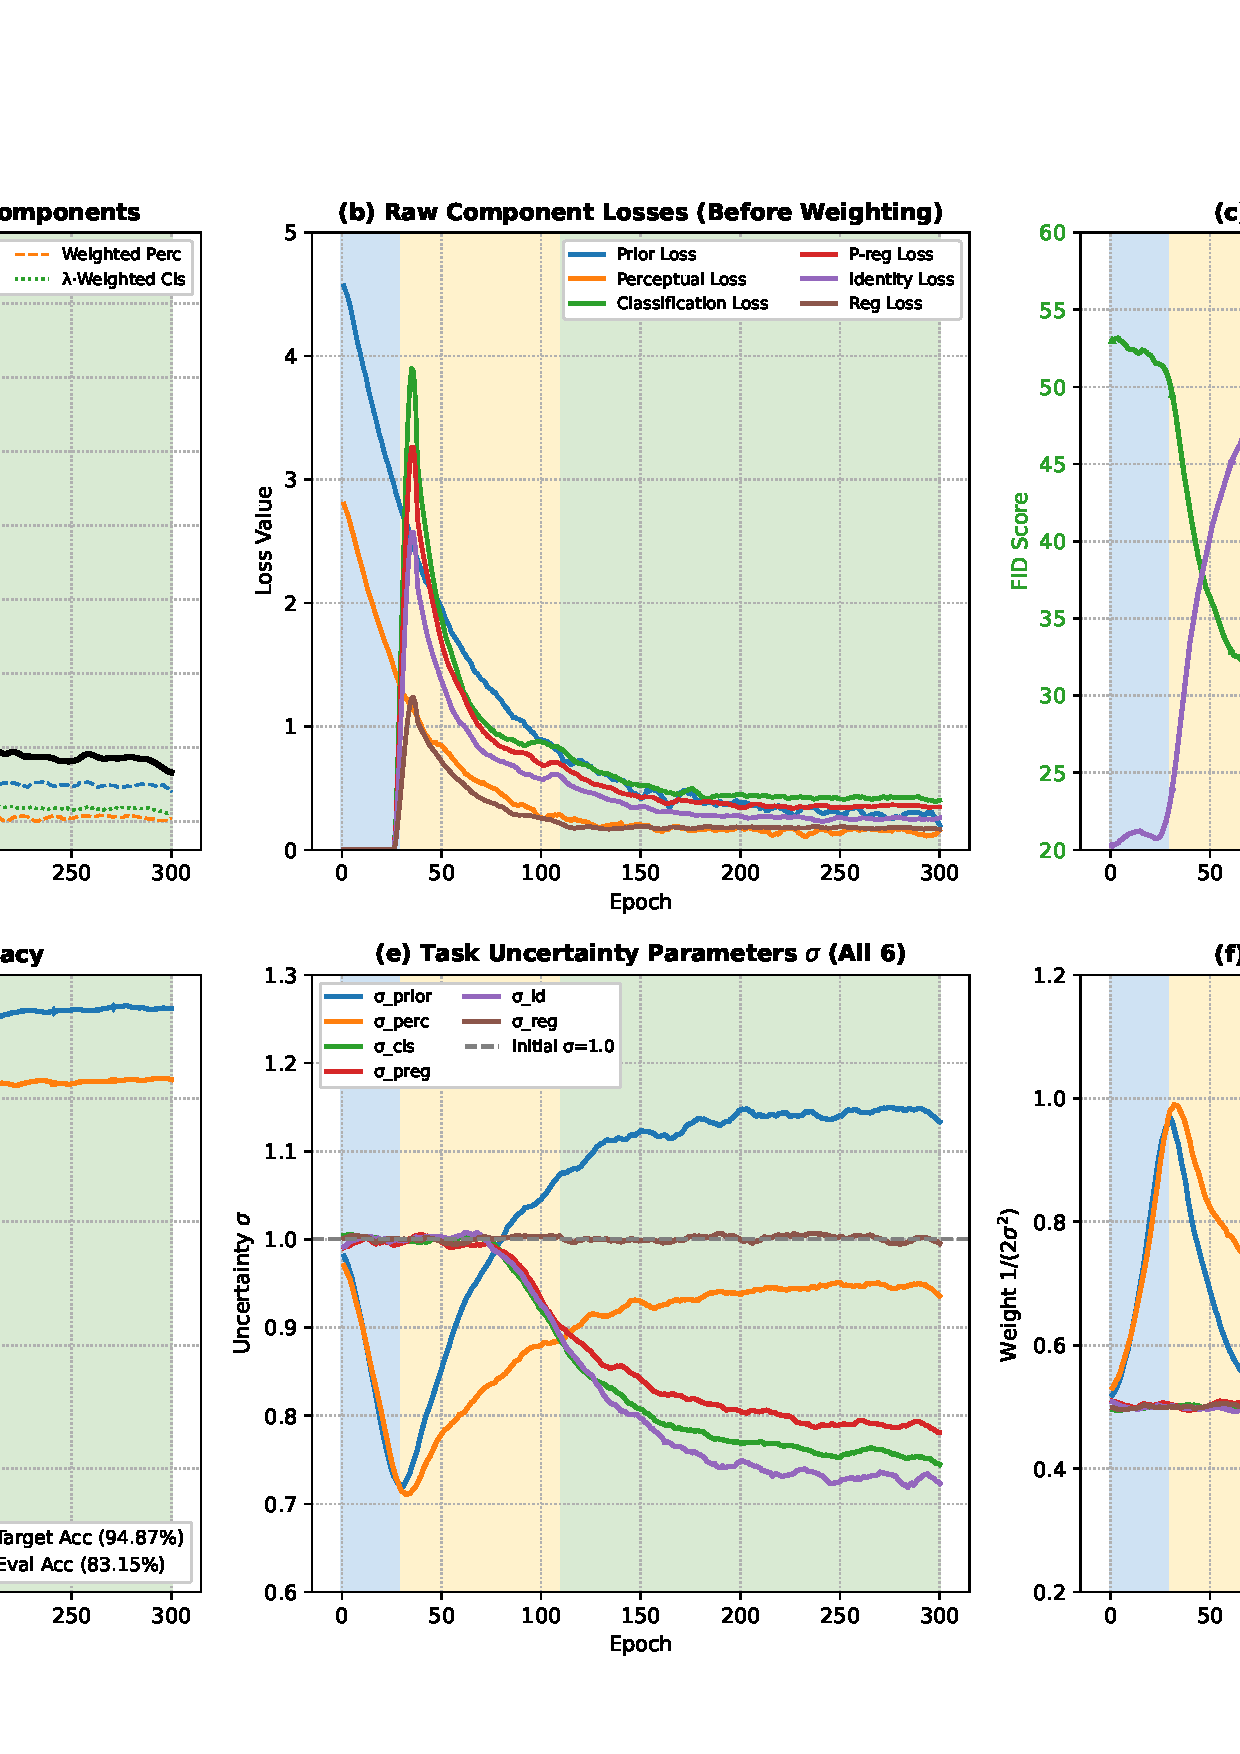
\includegraphics[height=0.48\textheight,keepaspectratio]{figures/mia_training_curves.pdf}\\
  {\scriptsize FID持续下降、KNN与准确率持续提升;\\不确定性参数动态调整实现多目标平衡}
\end{columns}
\end{frame} % 模型反演·消融实验分析

\section{研究结论}

\begin{frame}{研究总结}
\small

\begin{block}{基于角度约束对比学习的模板逆向重建方法}
\begin{itemize}
  \item 以EDM扩散模型为骨干,设计角度约束对比学习损失,精确对齐超球面决策边界
  \item 任务不确定性加权自动平衡多目标损失,模板条件梯度引导动态调整采样轨迹
  \item MOBIO攻击成功率97.38\%,LFW上FID=18.27
\end{itemize}
\end{block}

\vspace{0.2em}

\begin{block}{基于换脸先验迁移的多目标自适应模型反演方法}
\begin{itemize}
  \item 将扩散换脸模型应用于模型反演,通过标签条件嵌入层建立标签到身份的映射
  \item 渐进三阶段训练+LoRA参数高效微调
  \item 目标准确率94.87\%,评估准确率83.15\%,FID=23.26
\end{itemize}
\end{block}

\end{frame} % 研究总结

\begin{frame}{防御措施讨论}

\textbf{特征空间防御}
\begin{itemize}
\item \textbf{特征混淆:}破坏超球面几何结构,削弱角度约束对比学习的判别能力
\item \textbf{噪声注入:}在特征空间添加随机噪声,降低攻击的特征匹配精度
\end{itemize}

\vspace{0.4em}

\textbf{对抗训练防御}
\begin{itemize}
\item \textbf{对抗样本训练:}使用逆向重建样本对识别器进行对抗训练,提升模型鲁棒性
\item \textbf{正则化约束:}限制模型过度拟合,约束梯度信息的泄露程度
\end{itemize}

\vspace{0.4em}

\textbf{模型输出防御}
\begin{itemize}
\item \textbf{差分隐私机制:}在模型输出中添加校准噪声,干扰梯度信息获取
\item \textbf{置信度限制策略:}限制输出置信度范围,直接降低模型反演攻击有效性
\end{itemize}

\end{frame} % 防御措施讨论





\begin{frame}{专家评议意见及修改}
\footnotesize
\begin{enumerate}
\item  论文结论虽然提到了该成果在高安全阈值下攻击的成功率,但是并未讨论可能的防御手段对本文攻击有效性的影响。模型隐私性在业界获得了很高的关注度,也有若干防御措施提出。可讨论如何防御本文攻击或在有防御策略保护下本文攻击所受的影响。\\
\textcolor{hitblue}{在结论部分增加防御措施讨论}

\item  应规范术语及英文缩写的使用,如未给出"生成对抗网络(Generative Adversarial Network,GAN)"而直接使用"GAN"。\\
\textcolor{hitblue}{首次出现时提供全称及缩写,后续使用缩写形式。}

\item  论文第9页在章节安排中说明"本章在MOBIO、AgeDB和IJB-C等标准数据集上针对不同识别器架构进行系统实验验证",但第三章实际仅采用ArcFace一种架构进行实验,此处表述不够准确。\\
\textcolor{hitblue}{修正章节安排描述,确保与实际实验内容一致。}

\item  绪论部分引入较多变量与公式,建议简化或调整至后续章节,以保持引言部分的概括性与可读性。\\
\textcolor{hitblue}{将详细公式定义后移至第三四章,绪论中保留概念性描述。}

\end{enumerate}


\end{frame} % 专家评议意见及修改(第一页)

\begin{frame}{专家评议意见及修改}
\footnotesize
\begin{enumerate}
\setcounter{enumi}{4}

\item  第32页中,公式3-1所涉及的自然人脸分布($M_{natural}$)应进一步说明其与模板逆向攻击之间的关系,并解释为何样本$x$需满足该分布。\\
\textcolor{hitblue}{增加生成样本的自然性对于攻击成功率和隐蔽性的重要性表述。}

\item  章节3.3.1"整体架构设计"部分内容较为简略,建议补充网络结构细节及其功能说明,使整体设计更清晰完整。\\
\textcolor{hitblue}{增加架构设计的详细描述,包括各模块之间的数据流和功能说明。}

\item  表3-2在模型配置部分的描述应统一表述格式,以符合学术规范。\\
\textcolor{hitblue}{已修正相关表格和描述,确保格式一致且清晰。}

\item  图4-5应补充更详细的说明,特别是图像上方数字的含义,以便读者理解图示内容。\\
\textcolor{hitblue}{在图4-5的相关表述中增加对数字含义的解释,明确其为输入的标签类别。}

\item  结论部分可增加一段对未来研究方向的展望,以提升论文的完整性与启发性。\\
\textcolor{hitblue}{结论部分已包含一段全面的未来研究方向展望}

\end{enumerate}
\end{frame} % 专家评议意见及修改(第二页)

\end{document}
